\section{Resultados}\label{sec:resultados}

\subsection{\label{sub:data}Datos}\label{subsec:label{sub:data}datos}

Los datos de la elongaci�n del muelle 1 para distintas masas $m$ se muestran en la tabla~\ref{tab:1-y}.

El portamasas tiene un peso de 10\,g y se a�ade una masa inicial de 50\,g para tensar el muelle, por lo que $m_0 = 60$\,g.

El error absoluto asociado a las mediciones de las masas es $\pm 0.5$\,g.

El error absoluto asociado a las mediciones de las longitudes es $\pm 0.5$\,mm.

Estos errores se omiten de las tablas por claridad.


%Tabla
\begin{table}[tbh]
    \caption{Muelle 1 - Elongaci�n.}
    \label{tab:1-y}
    \begin{centering}
        \begin{tabular}{|P{37px}|P{53px}|P{37px}|P{53px}|}
            \hline
            $m$\,(g)  & $m + m_0$\,(g) & $y$\,(mm)  & $y - y_0$\,(mm)                       \\
            \hline
            \csvreader[late after line= \\]{./files/data/1-y.csv}{}% use head of csv as column names
            {\csvcoli & \csvcolii      & \csvcoliii & \csvcoliv}% specify your columns here
            \hline
        \end{tabular}
    \end{centering}
\end{table}


Las 3 mediciones para $n = 19$ oscilaciones se recogen en la tabla~\ref{tab:1-t1}.

\begin{table}[tbh]
    \caption{Muelle 1 - Tiempo.}
    \label{tab:1-t1}
    \begin{centering}
        \begin{tabular}{|P{27px}|P{26px}P{26px}P{26px}|P{26px}P{26px}|}
            \hline
            $m$\,(g)  & $t_1$\,(s) & $t_2$\,(s) & $t_3$\,(s) & $\langle t \rangle$\,(s) & $D_m$\,(s)                            \\
            \hline
            \csvreader[late after line= \\, /csv/separator=semicolon ]{./files/data/1-t1.csv}{}% use head of csv as column names
            {\csvcoli & \csvcolii  & \csvcoliii & \csvcoliv  & \csvcolv                 & \csvcolvi}% specify your columns here
            \hline
        \end{tabular}
    \end{centering}
\end{table}

En esta misma tabla, se han a�adido dos columnas adicionales. La columna $\langle t \rangle$ muestra la media de las 3 medidas
anteriores, o valor esperado de $t$, y la columna $D_m$ es la dispersi�n de los datos, calculada como:
\begin{equation}
    D_m = \frac{x_{\text{m�x}} - x_{\text{m�n}}}{2}
\end{equation}
La precisi�n del cron�metro era $0,01$\,s, un valor mucho menor que la dispersi�n $D_m$. Estos valores nos
sugieren que el error absoluto de las medidas de $t$ ser�a como m�ximo de $\pm 0.2$\,s.

La tabla~\ref{tab:1-t2} muestra de nuevo los valores de $t$ redondeados al n�mero de cifras significativas adecuado. Adem�s, se a�aden los valores del
periodo $T$ y su cuadrado $T^2$, con propagaci�n lineal de errores.

\begin{table}[tbh]
    \caption{Muelle 1 - Periodo.}
    \label{tab:1-t2}
    \begin{centering}
        \begin{tabular}{|P{56px}|P{67px}|P{67px}|}
            \hline
            $t$\,(s)   & $T = t / n$\,(s) & $T^2$\,(s)                            \\
            \hline
            \csvreader[late after line= \\, /csv/separator=semicolon ]{./files/data/1-t2(1).csv}{}% use head of csv as column names
            {\csvcolii & \csvcoliii       & \csvcoliv}% specify your columns here
            \hline
        \end{tabular}
    \end{centering}
\end{table}

\subsection{\label{sub:results}An�lisis}\label{subsec:label{sub:results}analisis}

\subsubsection{M�todo est�tico}

Representamos la deformaci�n $y-y_0$ frente a la masa $m$ en la figura~\ref{fig:r1}
y ajustamos los puntos a una recta de ecuaci�n $y = m\,x + b$,
donde $m = 0.424 $ y $b = -0.001$.
\footnote{En las figuras se emplea la notaci�n inglesa, siendo el punto el separador de decimales.
}.

\begin{figure}[tbh]
    \begin{center}
        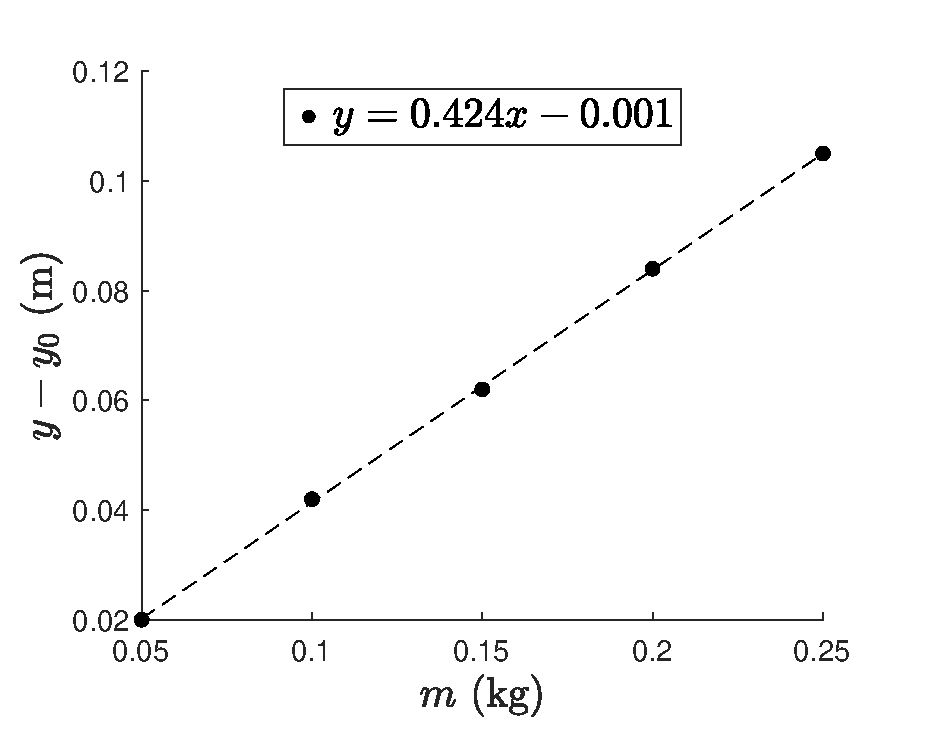
\includegraphics[width=0.8\columnwidth]{files/images/fig1}
    \end{center}
    \caption{Deformaci�n frente a masa.}
    \label{fig:r1}
\end{figure}

La desviaci�n est�ndar obtenida en la regresi�n lineal es $0.003$, por lo que tenemos:
\begin{equation*}
    \frac{g}{k_e} = (0.424 \pm 0.003)\, \text{m/kg}
\end{equation*}

Usando el valor de $g = (9.81 \pm 0.03)$\,m/s$^2$, obtenemos el valor de la constante el�stica calculada por el m�todo est�tico:
\begin{equation*}
    k_e = (23.1 \pm 0.2)\,\text{N} / \text{m}
\end{equation*}

El valor $b$ representa el corte de la recta con el eje de abscisas. En nuestro caso, ya que si no se cuelga ninguna masa del muelle
no hay elongaci�n, deber�a aproximarse al origen de coordenadas, como as� sucede.

\subsubsection{M�todo din�mico}

En la figura~\ref{fig:r2} se representa $T^2$ frente a $m+m_0$.

\begin{figure}[tbh]
    \begin{center}
        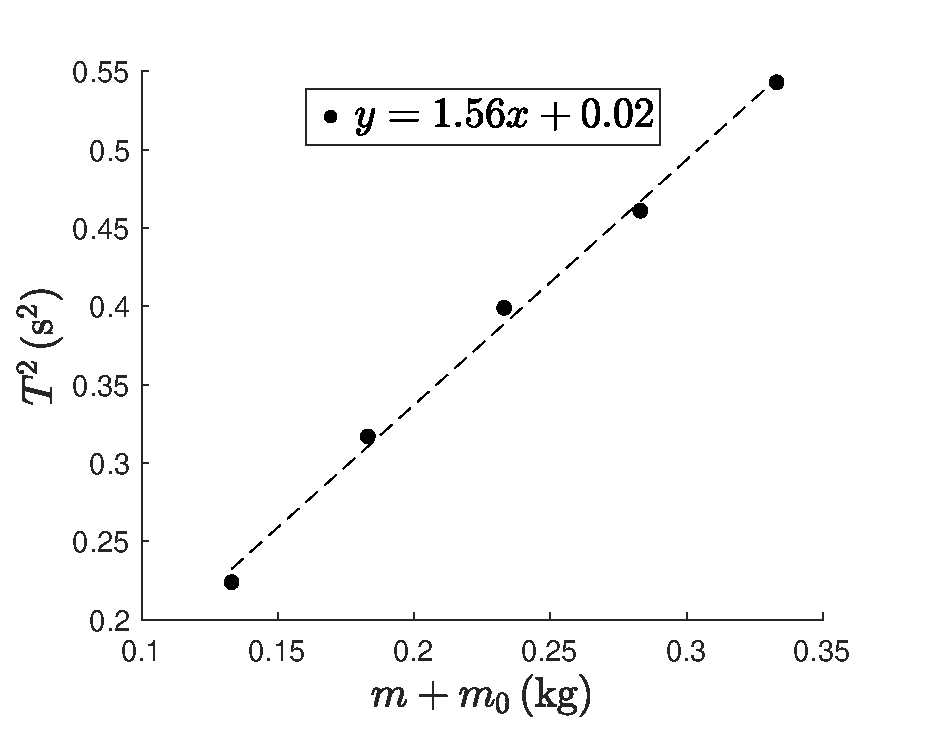
\includegraphics[width=0.8\columnwidth]{files/images/fig2}
    \end{center}
    \caption{Periodo al cuadrado frente a masa total.}
    \label{fig:r2}
\end{figure}

De la pendiente de la recta obtenemos:
\begin{equation*}
    \frac{4\pi^2}{k_d} = (1.56 \pm 0.06)\,\text{s$^2$/kg}
\end{equation*}

Por lo que el valor de la constante el�stica calculada por el m�todo din�mico es:
\begin{equation*}
    k_d = (25.3 \pm 0.9 )\,\text{N/m}
\end{equation*}

\subsubsection{Comparaci�n de los m�todos}

El error relativo suponiendo que el resultado correcto sea el est�tico es:
\begin{equation*}
    \epsilon_r = \frac{\abs{ k_d - k_e }}{k_e} \cdot 100 = 9.5\%
\end{equation*}

//TODO �Diferencias entre ambos m�todos desde un punto de vista experimental?

\subsubsection{Masa efectiva}

La coordenada en el origen de la recta es $0.024 \pm 0.014$.

El valor $\alpha$ es la fracci�n de la masa del muelle que se mueve en el movimiento oscilatorio.
Se espera que su valor se encuentre entre 0 y 1.